\documentclass[9pt]{article}
\usepackage[letterpaper,margin=0.48in]{geometry}
\usepackage[T1]{fontenc}
\usepackage{lmodern}
\usepackage{microtype}
\usepackage{graphicx}
\usepackage{xcolor}
\usepackage{enumitem}
\usepackage{titlesec}
\usepackage{booktabs}
\setlength{\parindent}{0pt}
\setlength{\parskip}{2pt}
\renewcommand{\baselinestretch}{0.96}\normalsize
\setlist[itemize]{leftmargin=13pt,itemsep=1pt,topsep=1pt}
\setlist[enumerate]{leftmargin=15pt,itemsep=1pt,topsep=1pt}
\titleformat{\section}{\small\bfseries\color{blue!45!black}}{}{0pt}{}[\vspace{-2pt}\hrule\vspace{2pt}]
\titlespacing*{\section}{0pt}{5pt}{2pt}
\pagestyle{empty}

\newcommand{\project}{\textit{The Secret Rhythm of the Ocean}}
\newcommand{\dist}{\(\sqrt{\sum_j(u_j-v_j)^2/d}\)}

\begin{document}
\vspace*{-10pt}
\begin{center}
{\Large\bfseries Distance-First Revision: Request for Feedback}\\[-1pt]
{\small \project\ --- Prachi Aswani, Jacob Erard, Parker Suzuki --- CS 6/5140 / DS 4140}
\end{center}
\vspace{-3pt}

\textbf{Why this revision.} Your feedback made clear that our earlier write-up
foregrounded PCA/K-means instead of the key data-mining choices: the object,
representation, distance, and structure found from that distance. PCA/K-means/GMM
are now reproducible baselines only.

\section*{What the raw data look like, and how an object becomes a vector}
The source file \texttt{Data Mining Project/all.csv} has \textbf{886,809 long-format
measurements}: one row for each \((\text{UTC timestamp},\text{deployment},\text{frequency band})\).
Each row contains a sound-level value; there are 33 one-third-octave frequency
bands per observed hour. We validate timestamps, duplicate time-frequency keys,
and complete spectra, then pivot the long table into \textbf{26,873 hourly vectors}.

\begin{center}\small
\fbox{\parbox{0.92\linewidth}{
\textbf{Raw long row:} \(t\), deployment, frequency (Hz), sound level (dB)\\
\(\downarrow\) pivot the 33 frequencies at the same hour\\
\textbf{Hourly spectrum:} \(x_t\in\mathbb{R}^{33}\) = [level at band 1, \ldots, level at band 33]\\
\(\downarrow\) keep 24 consecutive hourly spectra from one deployment\\
\textbf{Daily object:} \(X\in\mathbb{R}^{24\times33}\) (a matrix: rows = UTC hours; columns = frequency bands)\\
\(\downarrow\) transform and flatten, while preserving the fixed hour-band order\\
\textbf{Daily vector:} \(u=\mathrm{vec}(X)\in\mathbb{R}^{792}\), used only to calculate distances between days.}}
\end{center}

Only a complete, contiguous day from one deployment is retained. Partial days,
gaps, and deployment boundaries are excluded, leaving \textbf{1,101 daily objects}.

\section*{The two explicit acoustic distances}
For daily vectors \(u,v\) with \(d=24\times33=792\), both comparisons use RMS
Euclidean distance \dist. The meaningful modeling choice is what goes into the
vector:

\begin{itemize}
  \item \textbf{Level-sensitive:} standardize every frequency band over all
  observed hours, then flatten. This preserves absolute level and within-day
  evolution.
  \item \textbf{Shape-only:} subtract each hour's broadband mean before the
  same bandwise standardization and distance. Thus a loud and quiet version of
  the same spectral shape can be close.
\end{itemize}

Ship, weather, animal, calendar, and old cluster-state variables are \textbf{not}
in either distance. They are held out until after acoustic patterns are found.

\section*{Structure mined from the distance}
\begin{minipage}[t]{0.60\linewidth}
\begin{itemize}
  \item \textbf{Recurring motifs:} nearest daily neighbors at least 14 calendar
  days apart, so a day cannot simply match the day beside it.
  \item \textbf{Mutual-kNN neighborhoods:} days that select each other among
  their 10 closest shape-only neighbors.
  \item \textbf{Unusual days:} rank each day by its mean distance to its 10
  nearest non-overlapping days.
\end{itemize}
\textbf{Early check that the modeling choice matters:} the two representations
select the same rank-one neighbor for only \textbf{21.3\%} of days. Thus they do
not merely redraw the same clusters: level and spectral shape produce different
similarity decisions.
\end{minipage}\hfill
\begin{minipage}[t]{0.37\linewidth}
\vspace{-5pt}
\centering
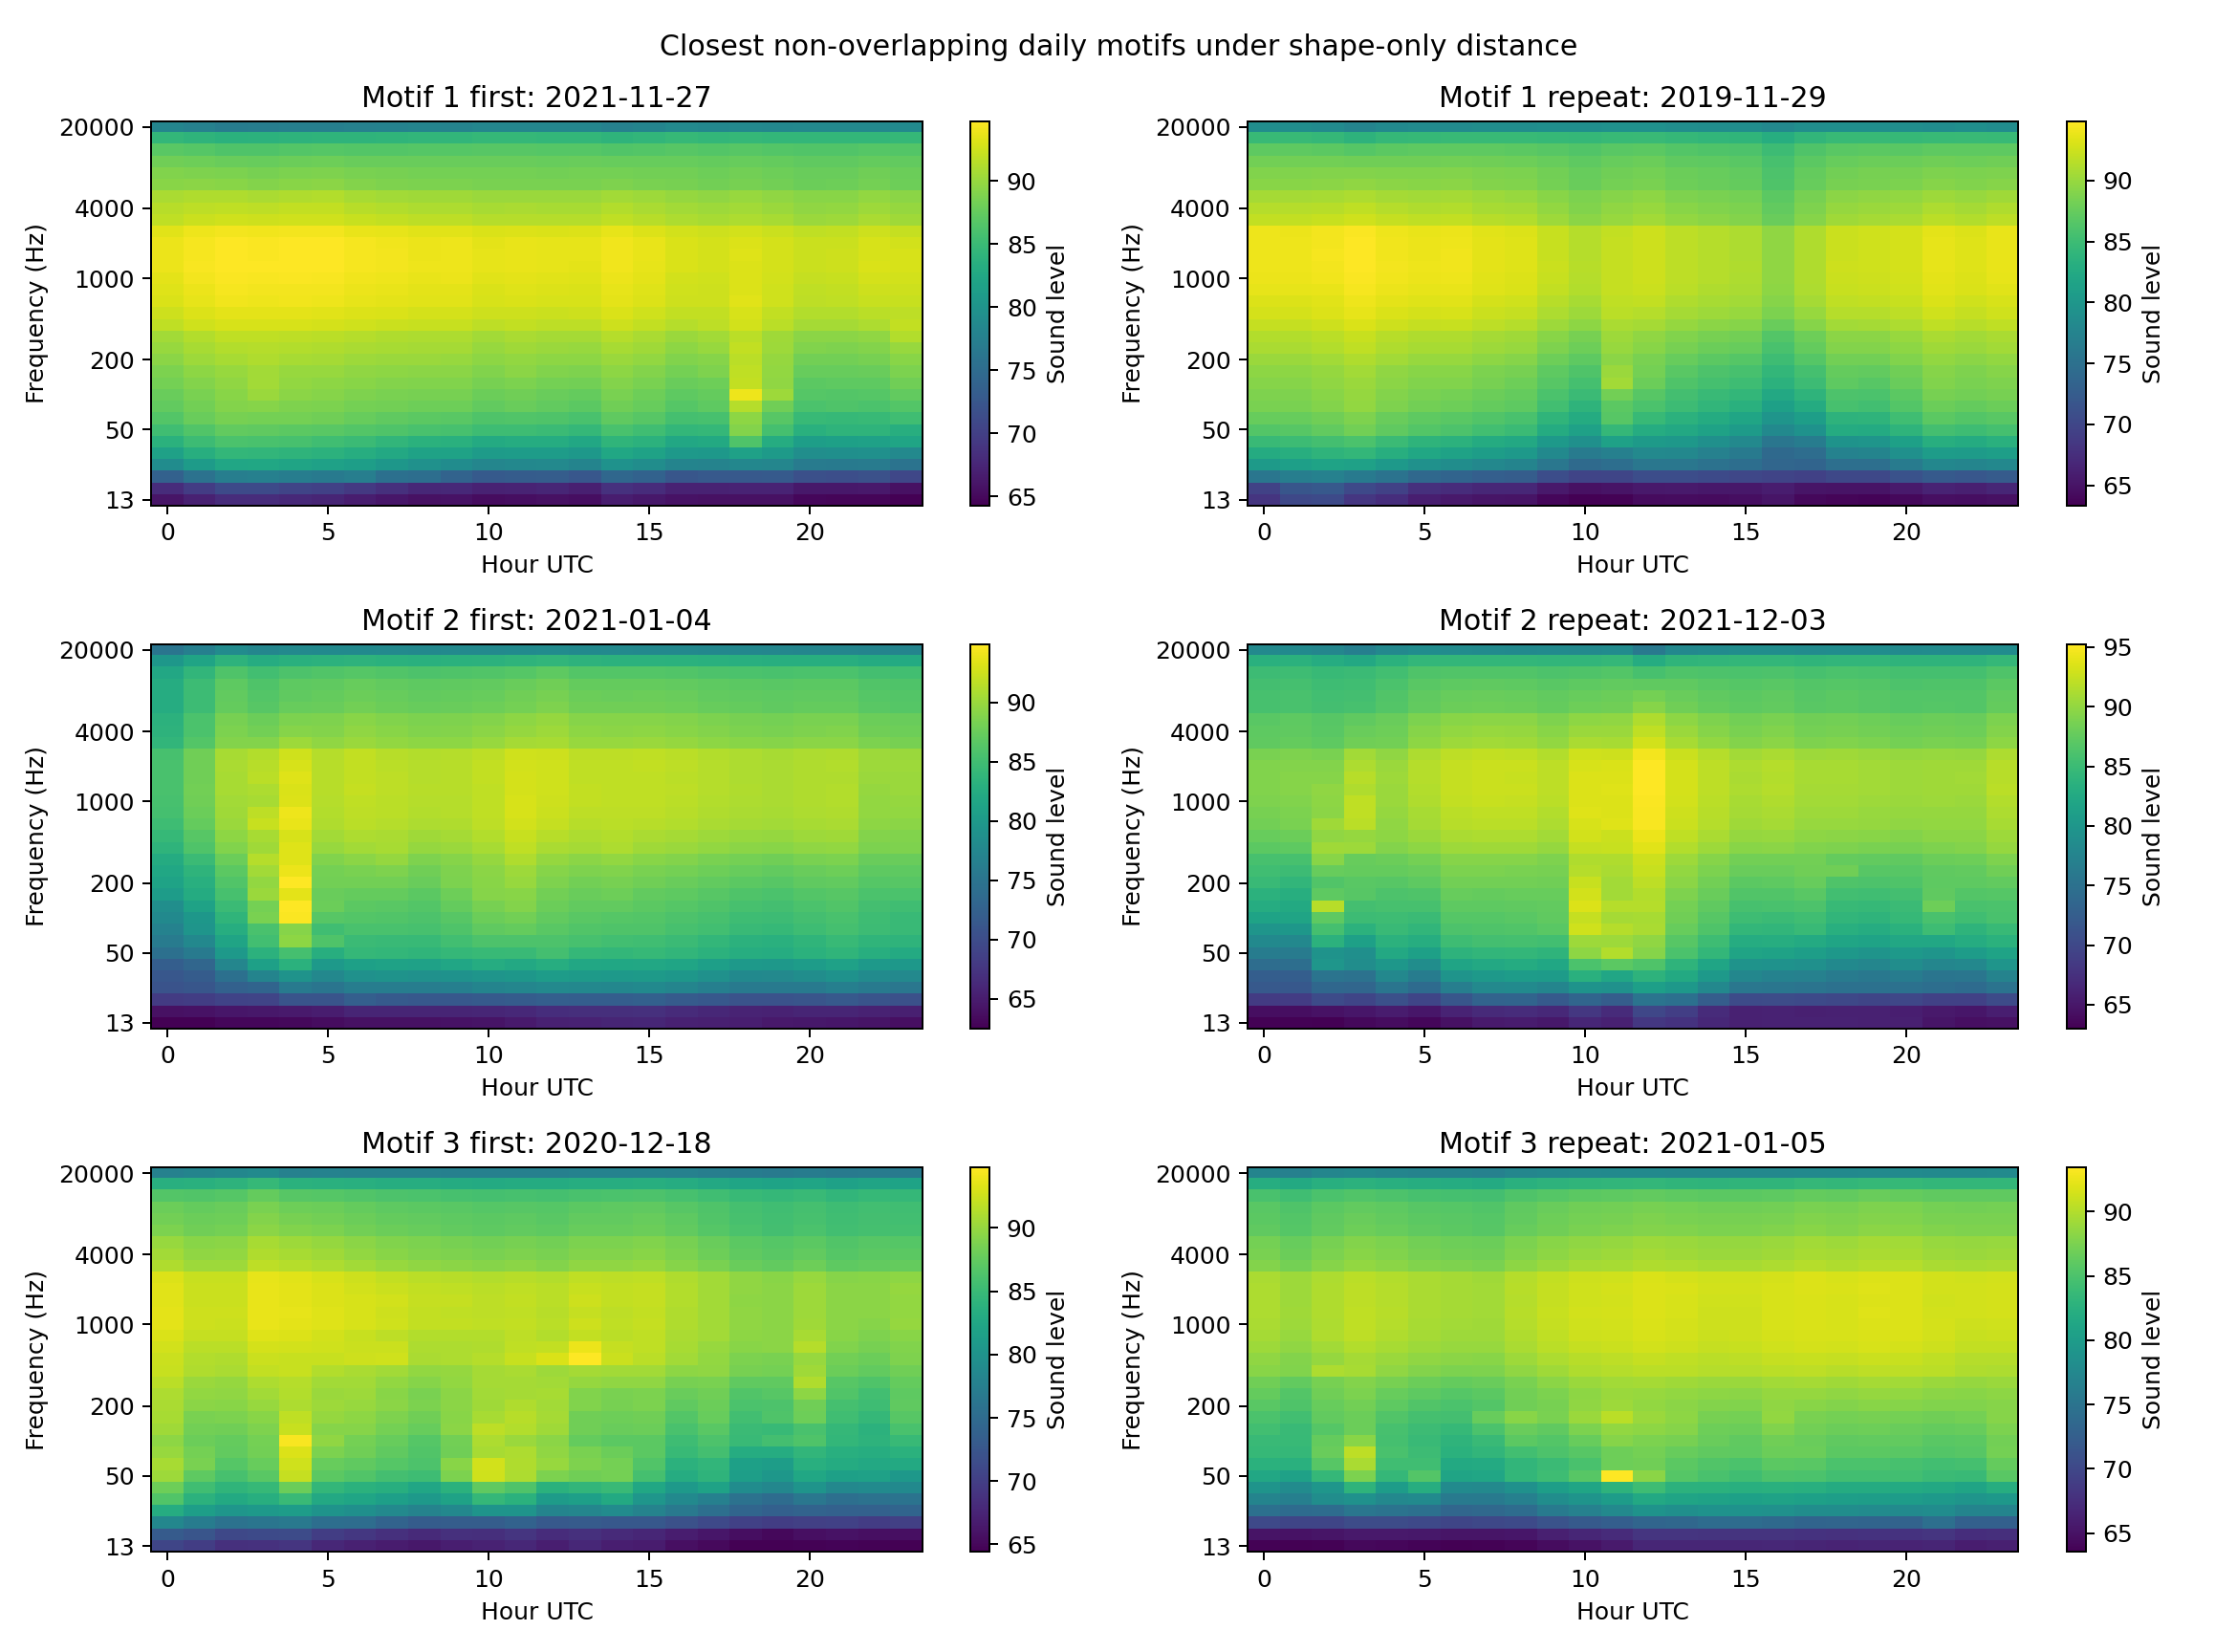
\includegraphics[width=\linewidth,height=2.00in,keepaspectratio]{../results/distance_first/figures/shape_only_daily_motifs.png}\\[-4pt]
{\scriptsize Closest non-overlapping shape-only motif pairs.}
\end{minipage}

\section*{Concrete preliminary examples (not causal claims)}
The closest shape-only repeated motif is \textbf{Nov. 27, 2021} (SB01\_18) and
\textbf{Nov. 29, 2019} (SB01\_06), distance \(0.283\). The leading shape-only
unusual day is \textbf{Oct. 2, 2020} (SB01\_12), mean 10-NN distance \(1.543\).
The next analysis step is to inspect those examples and only then compare their
held-out ship, weather, and animal context. We will not call an observed
association a cause without appropriate evidence.

\section*{Feedback we need before extending the analysis}
\begin{enumerate}
  \item Is a complete 24-hour matrix the right primary object, or should the
  main object instead be a 7-day acoustic sequence?
  \item Is this level-sensitive versus shape-only comparison a sufficiently
  meaningful distance-design experiment? If not, which alternative distance or
  representation would you expect us to compare?
  \item Do nearest-neighbor motifs, mutual-kNN neighborhoods, and
  distance-based outliers constitute the right kind of structure for this
  project? Would you want a time-series foundation-model embedding as an
  additional representation after this transparent baseline?
\end{enumerate}

\vfill
{\scriptsize Reproducibility: \texttt{python -m scripts.run\_distance\_first\_analysis}. Generated tables, distance matrices, and figures are in \texttt{results/distance\_first/}.}
\end{document}
